\documentclass{beamer}
\usepackage[T1]{fontenc}

\usepackage{polski}
\usepackage[utf8]{inputenc}
\usepackage[polish]{babel}
%
% Choose how your presentation looks.
%
% For more themes, color themes and font themes, see:
% http://deic.uab.es/~iblanes/beamer_gallery/index_by_theme.html
%
\mode<presentation>
{
	\usetheme{Warsaw}      % or try Darmstadt, Madrid, Warsaw, ...
	\usecolortheme{crane} % or try albatross, beaver, crane, ...
	\usefonttheme{default}  % or try serif, structurebold, ...
	\setbeamertemplate{headline}{}
	\setbeamertemplate{caption}[numbered]
} 

\title[Praca magisterska]{Rekomendacje artykułów opisujących produkty w serwisach e-commerce}
\author{Łukasz Dragan}
\institute{Informatyka spec. Metody sztucznej inteligencji, MiNI PW}
\date{31.10.2017}

\begin{document}
	
	\begin{frame}
		\titlepage
	\end{frame}
	
	\begin{frame}{Plan prezentacji}
	  \tableofcontents
	\end{frame}
	
	\section{Opis problemu}
	
	\begin{frame}{Cel pracy}
		Czy metody semantycznej analizy tekstu mogą być alternatywą dla~dotychczas używanej przez~\emph{Allegro} metody generowania rekomendacji artykułów tekstowych?
		%powiedzeić o swojej motywacji: nie znałem wcześniej tej tematyki, nie znałem Pani Promotor, temat wydał mi się ciekawy, bo było to realne biznesowe zastosowanie informatyki. Ostatecznie otworzyło to przede mną szerokie pole do dalszego zainteresowania tematem. A i współpraca okazała się owocna
	\end{frame}
	
	\begin{frame}{pracuj.pl}
		\begin{figure}
			\centering
			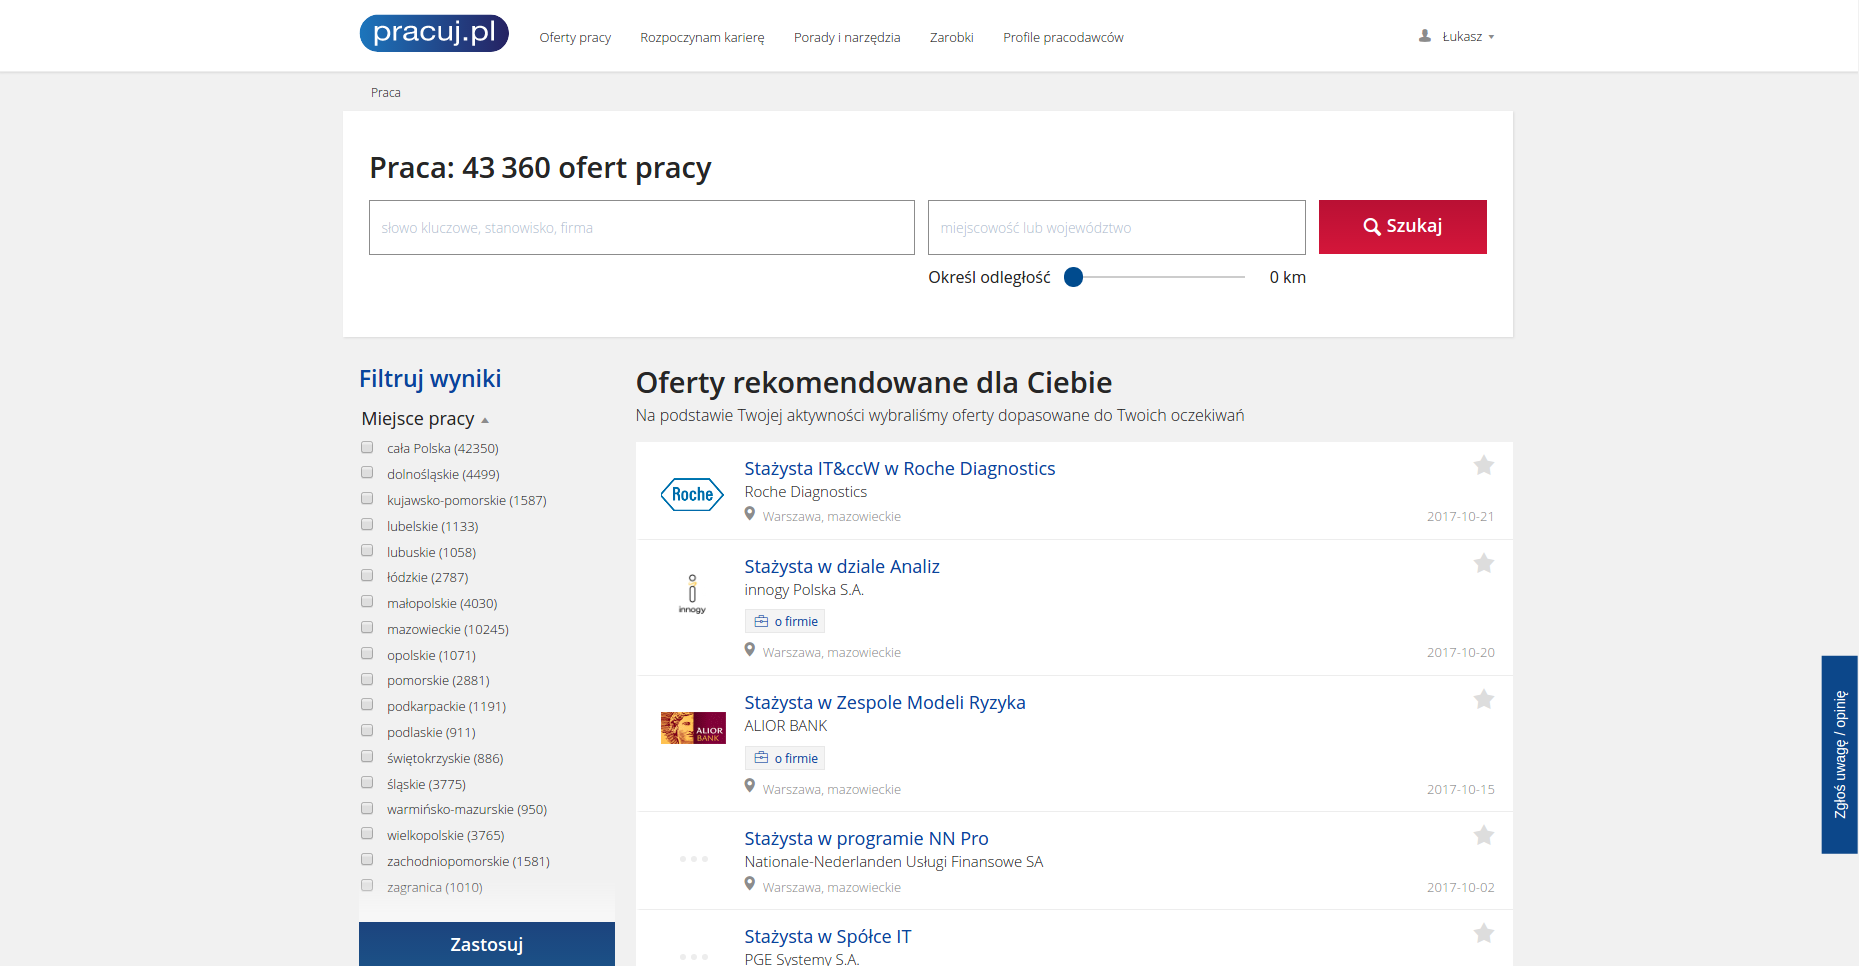
\includegraphics[width=1\textwidth]{img/pracuj.png}
		\end{figure}
	\end{frame}
	
	\begin{frame}{filmweb.pl}
		\begin{figure}
			\centering
			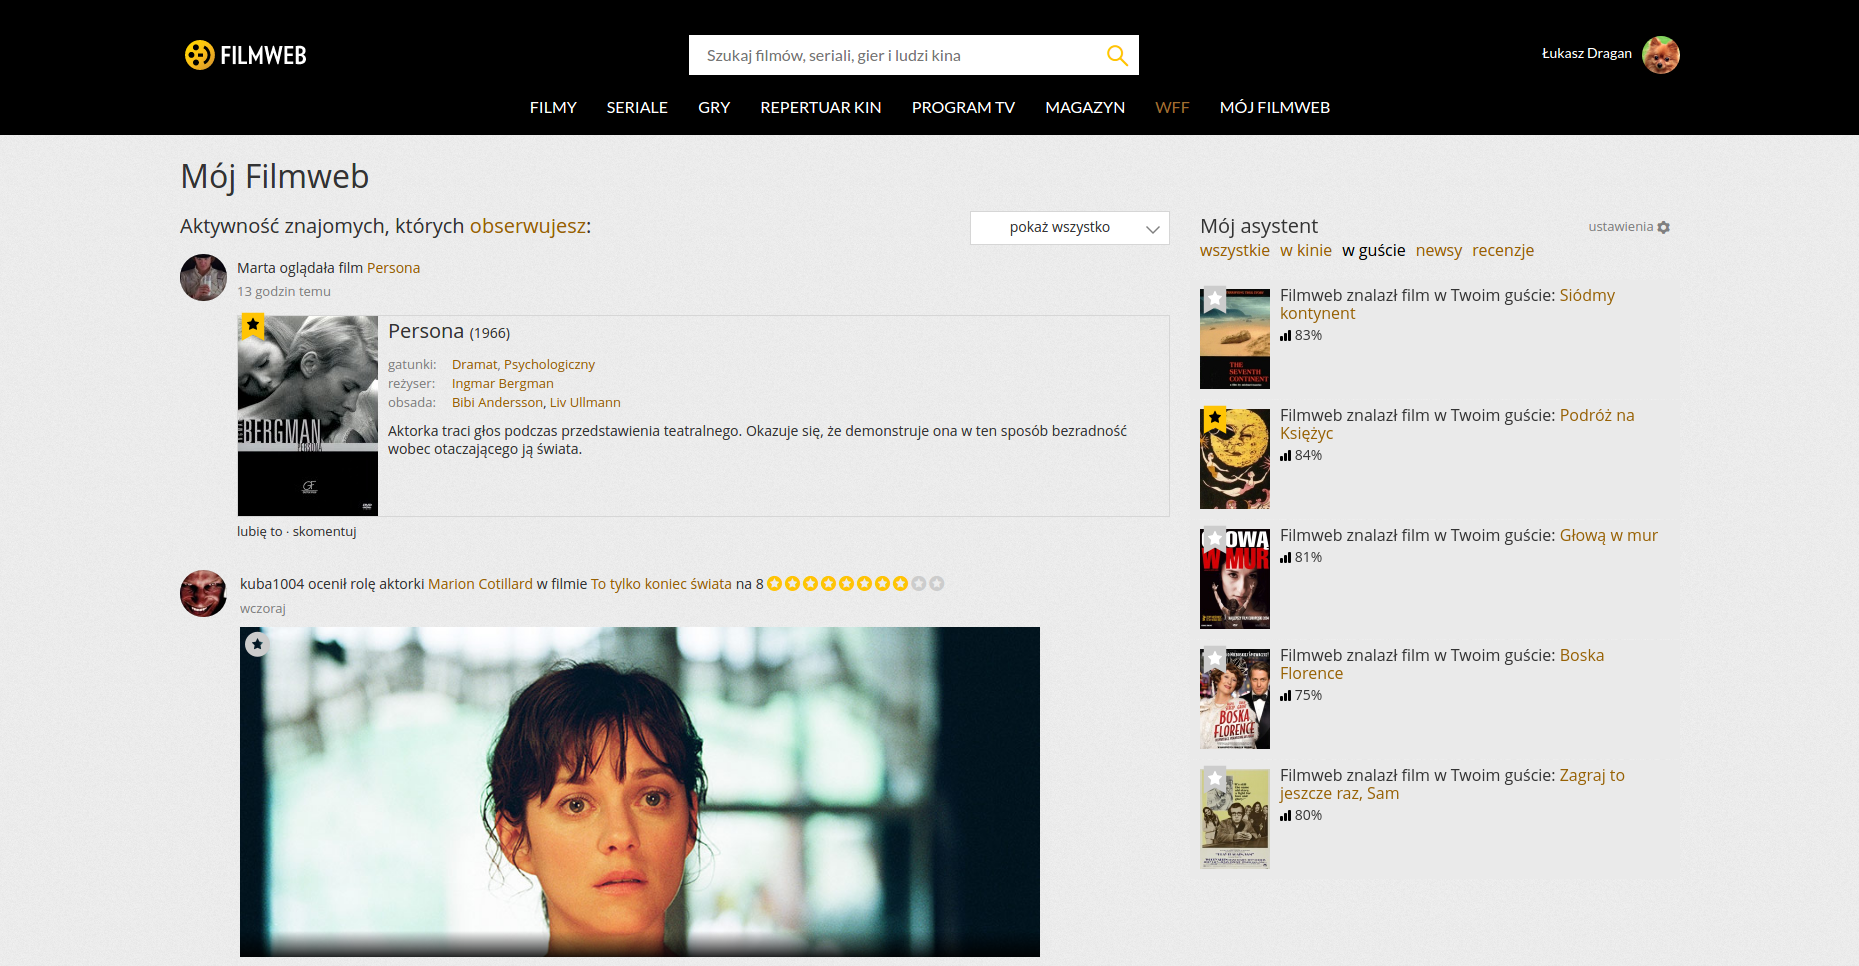
\includegraphics[width=1\textwidth]{img/filmweb.png}
		\end{figure}
	\end{frame}
	
	\begin{frame}{allegro.pl}
		\begin{figure}
			\centering
			
\includegraphics[width=1\textwidth]{img/screen_allegro.png}
		\end{figure}
	\end{frame}
	
	\begin{frame}{allegro.pl cd}
		\begin{figure}
			\centering
			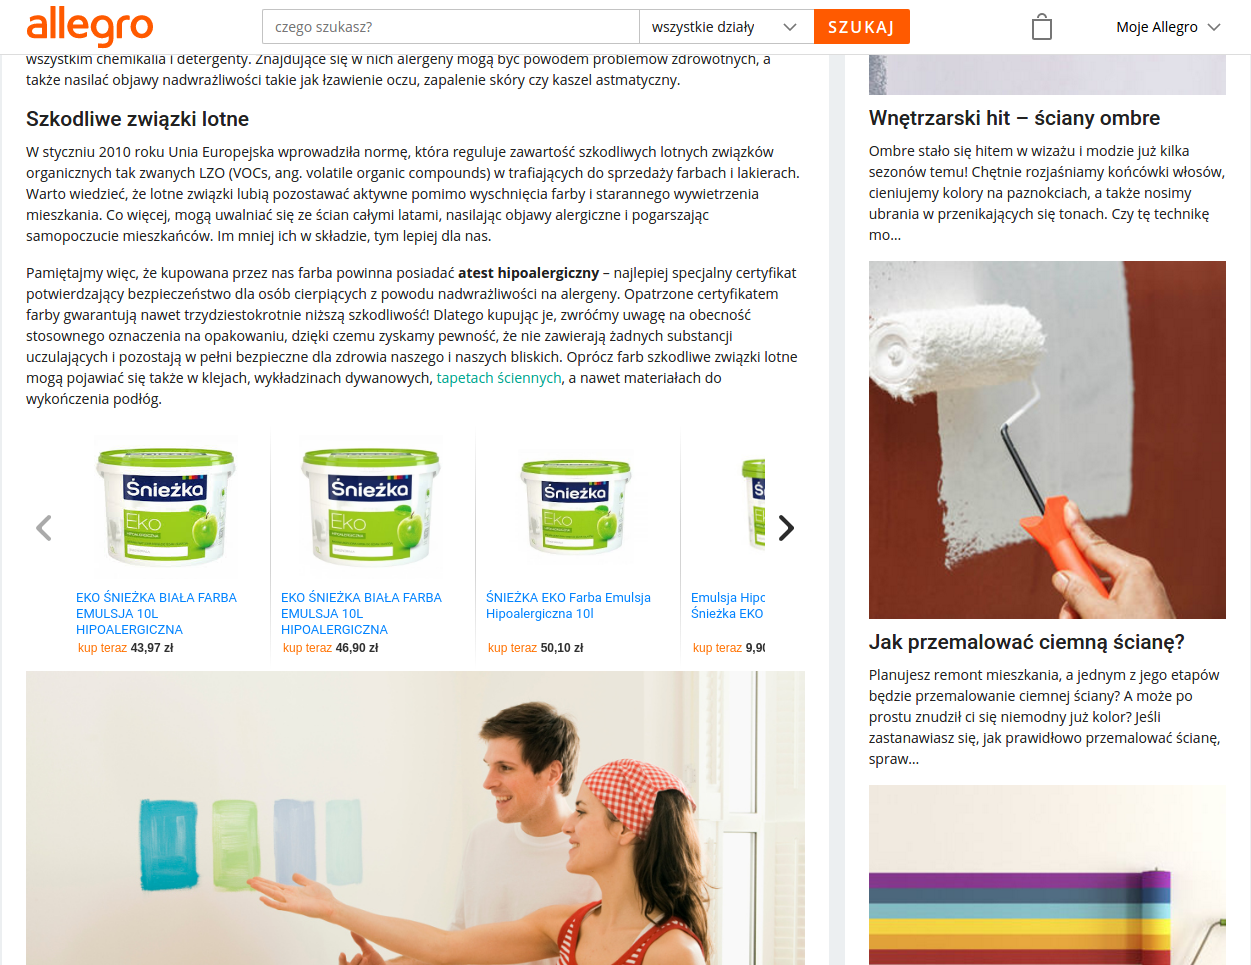
\includegraphics[width=1\textwidth]{img/screen_allegro_2.png}
		\end{figure}
	\end{frame}
	
	\section{Systemy rekomendacji}
	\begin{frame}{Elasticsearch}
		\begin{figure}
			\centering
			
\includegraphics[width=0.5\textwidth]{img/elastic-logo.png}
		\end{figure}
		,,Elasticsearch is a distributed, JSON-based search and analytics engine designed for horizontal scalability, maximum reliability, and easy management.''
	\end{frame}

	\begin{frame}{Systemy rekomenadacji}
		%TODO
		W ujęciu ogólnym systemy wyszukiwania mają na~celu sugerowanie tego, co użytkownik chciałby otrzymać. Natomiast systemy rekomendacji mają sugerować przedmioty potrzebne użytkownikowi nawet, jeżeli potrzeby te nie~zostały bezpośrednio wyrażone.
	\end{frame}
	
	\begin{frame}{Systemy rekomenadacji}
		\begin{figure}
			\centering
			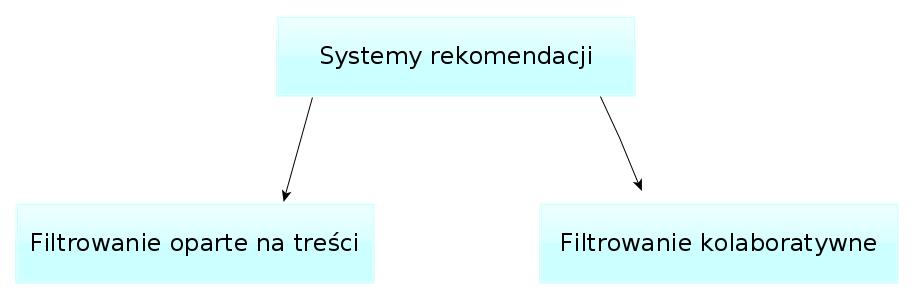
\includegraphics[width=1\textwidth]{img/recommender.png}
		\end{figure}
	\end{frame}
	\section{Techniki przetwarzania języka naturalnego}
	\begin{frame}{Zarys podejścia}
		\begin{figure}
			\centering
			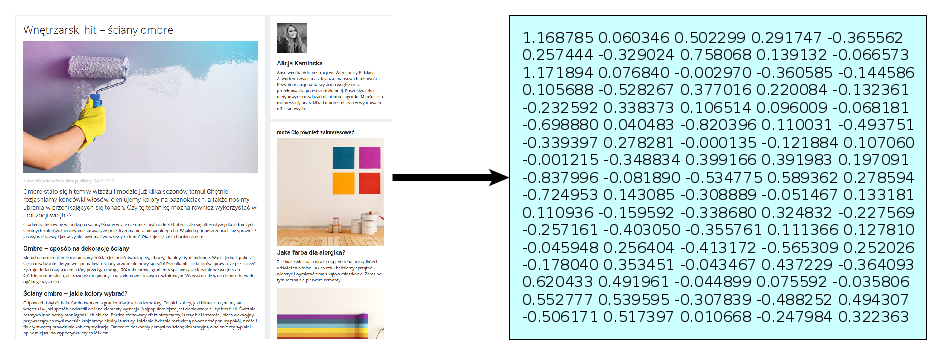
\includegraphics[width=0.85\textwidth]{img/approach_outline.png}
		\end{figure}
		\pause
		\begin{figure}
			\centering
			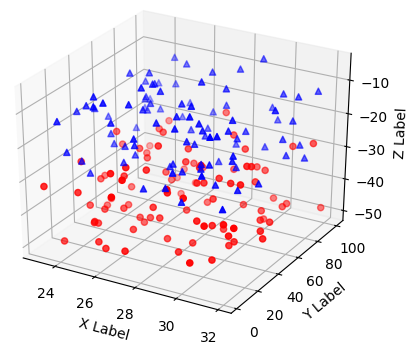
\includegraphics[width=0.45\textwidth]{img/scatter3d_demo.png}
		\end{figure}
	\end{frame}
	\begin{frame}{Dystans między wektorami}
		\begin{figure}
			\centering
			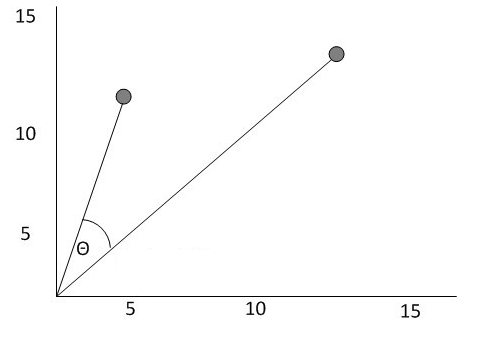
\includegraphics[width=0.6\textwidth]{img/cos.png}
		\end{figure}
		\pause % dyatans kosinusowy zwraca od razu znormalizowany wynik
		\begin{equation}
		\label{eq:cos}
		sim=\cos(\theta )={\frac {\sum \limits _{i=1}^{n}{A_{i}B_{i}}}{{\sqrt {\sum \limits _{i=1}^{n}{A_{i}^{2}}}}{\sqrt {\sum \limits _{i=1}^{n}{B_{i}^{2}}}}}},
		\end{equation}
		gdzie $A_i$ i $B_i$ są składowymi wektorów $A$ i $B$
	\end{frame}
	\begin{frame}{Bag-of-words}
		\begin{figure}
			\centering
			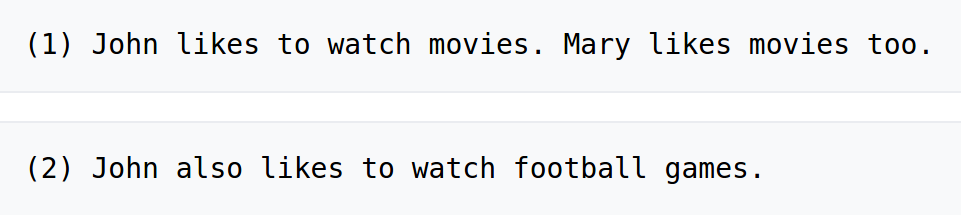
\includegraphics[width=0.75\textwidth]{img/bow_sents.png}
		\end{figure}
		\pause
		\begin{figure}
			\centering
			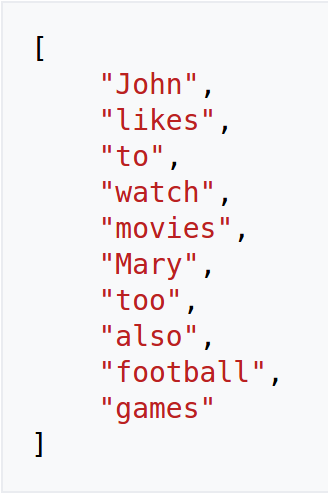
\includegraphics[width=0.25\textwidth]{img/bow_dict.png}
		\end{figure}
		\pause
		\begin{figure}
			\centering
			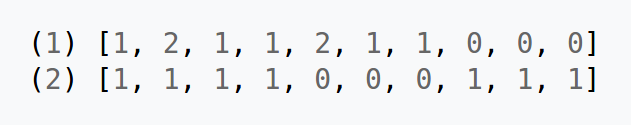
\includegraphics[width=0.5\textwidth]{img/bow_repr.png}
		\end{figure}
		% Wadą jest traktowanie każdego słowa z~jednakową wagą
	\end{frame}
	\begin{frame}{TF – term frequency, IDF – inverse document frequency}
		Wartość \textit{TF-IDF} słowa $w_i$ w dokumencie $d_j$:
		\begin{equation}
		\label{eq:tf-idf}
		tfidf_{ij} = tf_{ij} * idf_i,\ tf_{ij} = \frac{n_{ij}}{\sum\limits_{k}n_{kj}},\ idf_i = log\frac{|D|}{|{d:w_i \in d}|}
		\end{equation}
		\begin{itemize}
			\item $tf_{ij}$: liczba wystąpień słowa $w_i$ w~dokumencie $d_j$ podzielona przez~liczbę słów dokumentu $d_j$,
			\item $idf_i$: liczba dokumentów w~korpusie podzielona przez~liczbę dokumentów zawierających przynajmniej jedno wystąpienie słowa $w_i$.
		\end{itemize}
	\end{frame}
	\begin{frame}{TF-IDF}
		Zalety:
		\begin{itemize}
			\item prostota \pause
		\end{itemize}
		Wady:
		\begin{itemize}
			\item duża wymiarowość wektorów \pause
			\item wektory niemalże ortogonalne
		\end{itemize}
	\end{frame}
	\begin{frame}{Semantyka dystrybucyjna}
		Distributional hypothesis --- ,,słowa występujące w~tym samym kontekście niosą ze~sobą podobne znaczenie.''
		%Kolejne, bardziej zaawansowane, omawiane tu metody opierają się na~tzw. distributional hypothesis --- hipotezie zakładającej, że słowa występujące w~tym samym kontekście niosą ze~sobą podobne znaczenie. Sprzyja to zastosowaniu metod algebry liniowej jako narzędzia obliczeniowego oraz sposobu reprezentacji tekstu. Podstawowe podejście polega na~zgromadzeniu informacji o~rozkładzie słów w~dokumentach w~postaci wielowymiarowych wektorów, a~następnie wyodrębnieniu podobieństw pomiędzy~tymi wektorami, które świadczyłyby o~pewnych powiązaniach między reprezentowanymi słowami.
	\end{frame}
	\begin{frame}{Latent semantic indexing (1988)}
		\begin{itemize}
			\item Redukcja wymiarowości macierzy wystąpień słów w~dokumentach
			\begin{center}
				\begin{tabular}{ | l | l | l | l | l | l | l |}
					\hline
					 & $d_1$ & $d_2$ & $d_3$ & $d_4$  & $d_5$  & $d_6$ \\ \hline
					statek & 1 & 0 & 1 & 0 & 0 & 0 \\ \hline
					łódź & 0 & 1 & 0 & 0 & 0 & 0 \\ \hline
					ocean & 1 & 1 & 0 & 0 & 0 & 0 \\ \hline
					podróż & 1 & 0 & 0 & 1 & 1 & 0 \\ \hline
					wycieczka & 0 & 0 & 0 & 1 & 0 & 1 \\
					\hline
				\end{tabular}
			\end{center}
			\item Hiperparametr: docelowa wymiarowość
		\end{itemize}
	\end{frame}
	\begin{frame}{Latent semantic indexing (1988)}
		\begin{itemize}
			\setlength\itemsep{3em}
			\item Rozkład według wartości osobliwych:
				\begin{equation}
				\label{eq:svd}
				A = U \Sigma V^T,\!
				\end{equation}
				$U$ i $V$ to macierze ortogonalne\\
				$\Sigma$ to macierz diagonalna, taka, że $\Sigma = diag(\sigma_i)$, gdzie $\sigma_{i}$, to~nieujemne wartości szczególne macierzy $A$.\pause
				% Wartości osobliwe σi macierzy A sa definiowane jako σi = √λ_i, gdzie λ_i oznacza wartości własne macierzy A∗A.
				%macierz ortogonalna: U^-1 = U^T 
			\item 
			\{(statek), (łódź), (ocean)\} $\to$ \\\{(1.3452 $*$ statek $+$ 0.2828 $*$ łódź), (ocean)\}
		\end{itemize}
	\end{frame}
	\begin{frame}{Latent Dirichlet allocation (2003)}
		\begin{itemize}
			\item Automatyczne wykrywanie tematów zawartych w dokumentach
			\item Dokumenty jako mieszanki tematów
			\item Tematy jako rozkłady prawdopodobieństwa na zbiorze słów
			\item Hiperparametr: docelowa liczba tematów
		\end{itemize}
	\end{frame}
	\begin{frame}{Latent Dirichlet allocation (2003)}
		Algorytm --- próbkowanie Gibbsa:\\
		\begin{enumerate}
			\setlength\itemsep{2em}
			\item Przejdź przez każdy dokument i~losowo (zgodnie z~rozkładem Dirichleta) przypisz każde słowo dokumentu do~jednego z $T$ tematów.
			% Warto zauważyć, iż etap ten daje pierwsze	przybliżenie docelowej reprezentacji. W kolejnych krokach należy poprawiać to przybliżenie.
			
			% Cechy rozkładu sprawiają, że tak dobrane początkowe wartości parametrów modelu są zgodne z intuicją, że dokument pokrywa jedynie mały zestaw tematów, a temat zawiera najczęściej tylko mały zestaw słów.
			\item Dla każdego dokumentu $d$, dla~każdego słowa $w$ należącego do~$d$, dla każdego tematu $t$ oblicz: $p(t | d)$
			%czyli odsetek liczby słów w $d$, które są aktualnie przypisane do tematu $t$
			oraz oblicz $p(w | t)$
			% czyli odsetek liczby wystąpień słowa $w$, które są przypisane do~tematu $t$ w~skali całego korpusu.
			Przypisz słowu $w$ nowy temat poprzez losowanie z~prawdopodobieństwem $p(t_i|d)*p(w|t)$ dla~każdego tematu $t_i$.
		\end{enumerate}
		% After repeating the previous step a large number of times, you’ll eventually reach a roughly steady state where your assignments are pretty good. So use these assignments to estimate the topic mixtures of each document (by counting the proportion of words assigned to each topic within that document) and the words associated to each topic (by counting the proportion of words assigned to each topic overall).
		
	\end{frame}
	\begin{frame}{Word embeddings}
		\begin{itemize}
			\item Osadzanie słów w przestrzeni wektorowej
			\item Uczenie nienadzorowane
			\item Niska wymiarowość wektorów
			\item Reprezentacja słów wraz z~zależnościami pomiędzy nimi
		\end{itemize}
		\pause
		% Dzieje się to w opozycji do wcześniejszych podejść podobnych do bag-of-words — produkującego ogromne, rzadkie wektory, których wymiary równają się rozmiarowi		słownika, o który oparty jest model (rzędu setek tysięcy)
		\begin{figure}
			\centering
			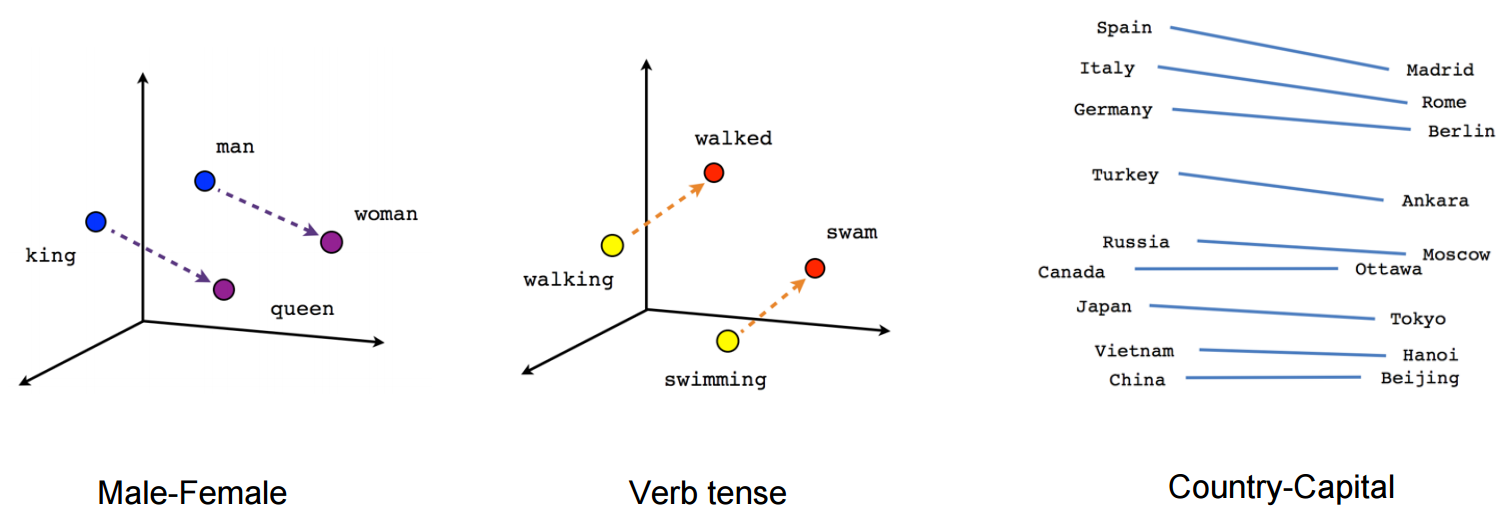
\includegraphics[width=1\textwidth]{img/linear-relationships.png}
		\end{figure}
		%https://www.tensorflow.org/images/linear-relationships.png
	\end{frame}
	\begin{frame}{Word2vec (2013)}
		płytkiej sieci neuronowej typu feed-forward
		\begin{figure}[H]
			\centering
			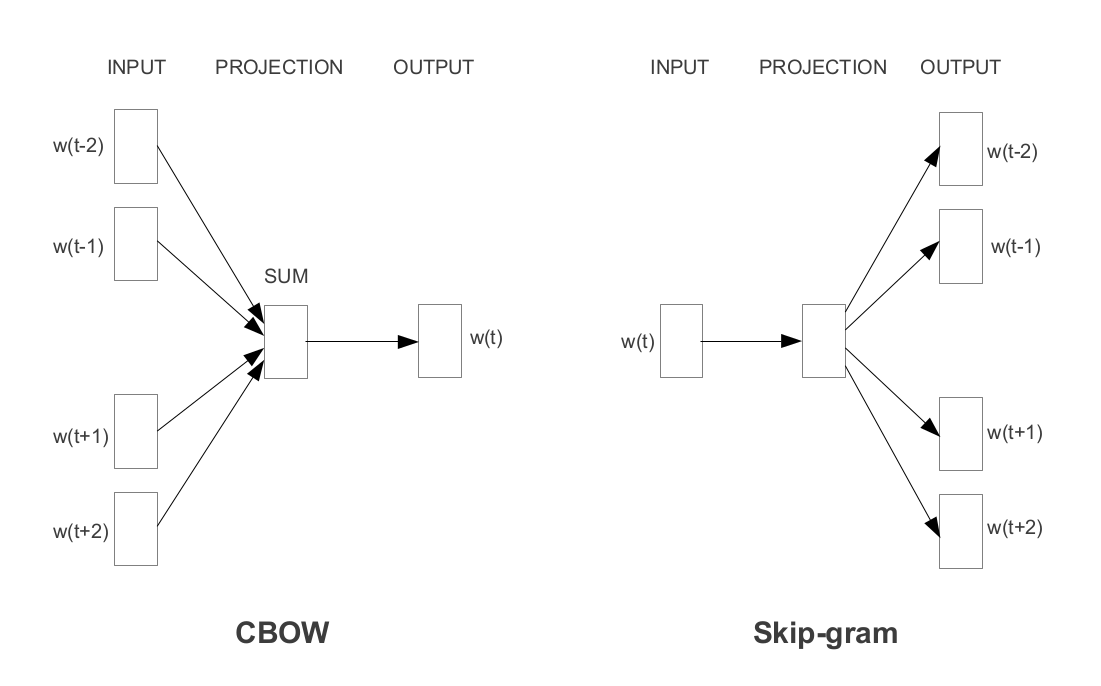
\includegraphics[width=0.9\textwidth]{img/skipgram_cbow.png}
			%\label{fig:warstwy}
		\end{figure}
	\end{frame}
	\begin{frame}{FastText (2017)}
		
	\end{frame}
	\begin{frame}{GloVe (2014)}
		\begin{itemize}
			\item Globalna macierz współwystąpień słów.
			% w przeciwieństwie do word2vec wykorzystuje informację o globalnym rozkładzie słów
			Ile razy słowo $w_i$ występuje w kontekście słowa $w_j$
			
		\end{itemize}



\begin{enumerate}
	\item Zgromadź współwystąpienia słów w formie macierzy $X$. Każdy element $X_{ij}$ takiej macierzy reprezentuje jak często słowo $i$ występuje w pobliżu słowa $j$. Zazwyczaj macierz buduje się poprzez skanowanie bazowego korpusu oknem o ustalonej szerokości, w obrębie którego centralne słowo leży w kontekście słów je otaczających. Dodatkowo można tu wprowadzić wagi dla słów malejące wraz ze wzrostem dystansu od słowa centralnego.
	\item Zdefiniuj ograniczenie dla każdej pary słów: $w_i^Tw_j + b_i + b_j = log(X_{ij})$, gdzie $w_i$ oznacza wektor głównego słowa, $w_j$ słowa leżącego w pobliżu $i$, $b_i$ i $b_j$ to skalary.
	\item Zdefiniuj funkcję kosztu \ref{eq:glove_loss}:
	\begin{equation}
	\label{eq:glove_loss}
	J = \sum_{i=1}^V \sum_{j=1}^V \; f(X_{ij}) ( w_i^T w_j + b_i + b_j - \log X_{ij})^2,
	\end{equation}
	gdzie f jest funkcją ważącą, która pomaga zapobiec uczeniu tylko na~podstawie najbardziej popularnych par słów. Autorzy proponują funkcję postaci \ref{eq:glove_loss_impl}:
	\begin{equation}
	\label{eq:glove_loss_impl}
	f(X_{ij}) = 
	\begin{cases}
	(\frac{X_{ij}}{x_{max}})^\alpha & \text{if } X_{ij} < XMAX \\
	1 & \text{w p.p.}
	\end{cases}
	\end{equation}
	Celem funkcji optymalizacji funkcji	 kosztu jest minimalizacja różnicy pomiędzy iloczynami skalarnymi wektorów współwystępujących słów.
	\item Dokonaj minimalizacji funkcji kosztu poprzez stopniową aktualizację wektorów $w_i$ i $w_j$.
\end{enumerate}
	\end{frame}

	\begin{frame}{Centroid}
		\begin{figure}
			\centering
			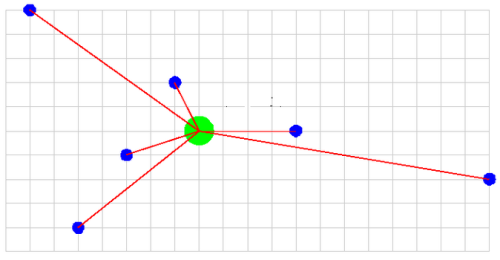
\includegraphics[width=1\textwidth]{img/centroid.png}
		\end{figure}
	\end{frame}
	\begin{frame}{Word Mover's Distance}
		Dystans pomiędzy dokumentami $A$ i $B$ to minimalny skumulowany dystans jaki słowa dokumentu $A$ muszą ,,przebyć'', aby osiągnąć słowa dokumnetu $B$
		\begin{figure}
			\centering
			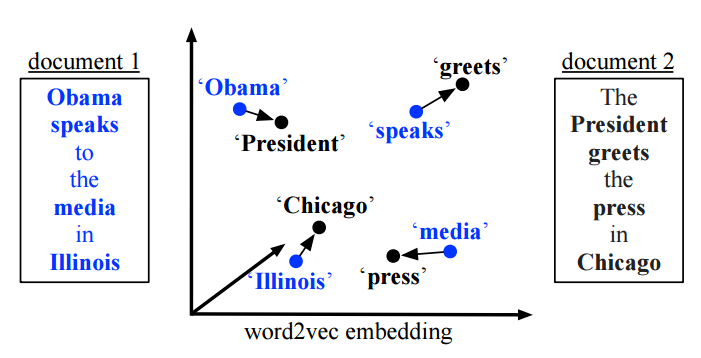
\includegraphics[width=1\textwidth]{img/wmd.png}
		\end{figure}
	\end{frame}
	\begin{frame}{Analiza danych}
		\begin{itemize}
			\item 20000~artykułów tekstowych w~formacie \textit{JSON}
			\item język polski
			\item słowa specyficzne dla różnych branż
			% ,,hipertoniczny'', ,,autofocus''
			\item struktura artykułu:
			\begin{itemize}
				\item treść: tytuł, nagłówek, tekst
				\item metadane: id, kategoria, słowa kluczowe
			\end{itemize}
			% w pracy opisuję dokładne statystyki
		\end{itemize}
	\end{frame}
	\begin{frame}{Wstępne przetwarzanie danych}
		\begin{enumerate}
			\item Oczyszczanie tekstu ze znaczników \pause
			\item Usunięcie słów stopu
		\end{enumerate}
	\end{frame}
	\begin{frame}{Słowa stopu}
		a, aby, ach, acz, aczkolwiek, aj, albo, ale, ależ, ani, aż, bardziej, bardzo, bo, bowiem, by, byli, bynajmniej, być, był, była, było, były, będzie, będą, cali, cała, cały, ci, cię, ciebie, co, cokolwiek, coś, czasami, czasem, czemu, czy, czyli, daleko, dla, dlaczego, dlatego, do, dobrze, dokąd, dość, dużo, dwa, dwaj, dwie, dwoje, dziś, dzisiaj, gdy, gdyby, gdyż, gdzie, gdziekolwiek, gdzieś, go, i...
	\end{frame}
	\begin{frame}
		\begin{enumerate}
			\item Oczyszczanie tekstu ze znaczników
			\item Usunięcie słów stopu \pause
			\item Zamiana na małe litery \pause
			% większości duże litery na początku zdania przeszkadzają, ale czasem wyraz z dużej litery i z małej znaczą co innego - Włochy
			\item Tokenizacja i lematyzacja % morfologik.blogspot.com
		\end{enumerate}
	\end{frame}
	\begin{frame}{Preprocessing - przykład}
		\begin{figure}
			\centering
			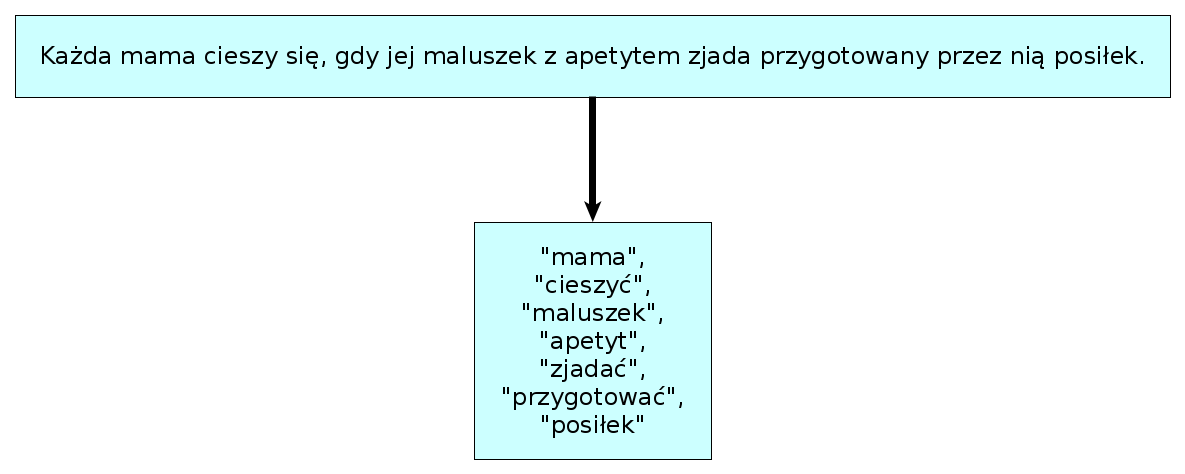
\includegraphics[width=1\textwidth]{img/lemmatisation.png}
		\end{figure}
	\end{frame}
	% jaka byłaby sytuacja idealna? zaaplikować rozwiązania w żywym systemie i porównać kpi
	\section{Metody ewaluacji}
	\begin{frame}{Miara jakości wyszukiwania: Normalized Discounted Cumulative Gain}
		\begin{itemize}
			\item Discounted Cumulative Gain:
			\begin{equation}
			\label{eq:dcg}
			{\mathrm  {DCG_{{p}}}}=\sum _{{i=1}}^{{p}}{\frac  {rel_{i}}{\log _{{2}}(i+1)}},
			\end{equation}
			gdzie $p$ to liczba elementów rankingu, $i$ to miejsce przedmiotu w~rankingu, a $rel$ to poziom relewantności elementu.
			%% DCG premiuje relewantne przedmioty, które są wysoko w~rankingu oraz~karze za~relewantne przedmioty w~dole rankingu. W~wariancie nDCG następuje jeszcze normalizacja przez~podzielenie wartości DCG rzeczywistego rankingu przez DCG idealnego rankingu ($IDCG$, \ref{eq:idcg}) zbudowanego na~elementach korpusu ułożonych malejąco pod~kątem relewantności.
			
			% im bardziej relewantne wyniki, tym wyżej powinny być w~rankingu, aby ranking był najbardziej wartościowy
			\pause
			\item Normalized Discounted Cumulative Gain:
			\begin{equation}
			\label{eq:ndcg}
			{\mathrm  {nDCG_{{p}}}}={\frac  {DCG_{{p}}}{IDCG_{{p}}}}.
			\end{equation}
		\end{itemize}
	\end{frame}
	\begin{frame}{Liczba wspólnych kategorii}
	\end{frame}
	\begin{frame}{Liczba wspólnych słów kluczowych}
	\end{frame}
	\begin{frame}{Kliknięcia użytkowników serwisu}
		\textit{clicks} --- ocena na~podstawie historycznej aktywności użytkowników mierzona na~podstawie liczby kliknięć w~odnośniki.
	\end{frame}
	\
	\begin{frame}{Ocena użytkowników offline}
		\begin{enumerate}
			\item \textit{mut\_kw[\_ndcg]} --- relewantność wyszukanych artykułów liczona na~podstawie liczby wspólnych słów kluczowych z~artykułem bazowym. Również stosuję dwa warianty: średnia relewantność wyszukanych artykułów oraz~miara \textit{nDCG}.
			\item \textit{users} --- ocena na~podstawie eksperckiej oceny użytkowników. W~badaniu wykorzystałem 5~użytkowników operujących każdy na~tym samym zbiorze par testowych. Pary zostały wygenerowane (zgodnie z~wcześniejszym opisem metody) na~podstawie 50 artykułów bazowych wylosowanych spośród wszystkich artykułów udostępnionych mi przez~\textit{Allegro}.
		\end{enumerate}
	\end{frame}
	\section{Testy}
	\begin{frame}{LSI w zależności od liczby tematów}
		\begin{figure}[H]
			\centering
			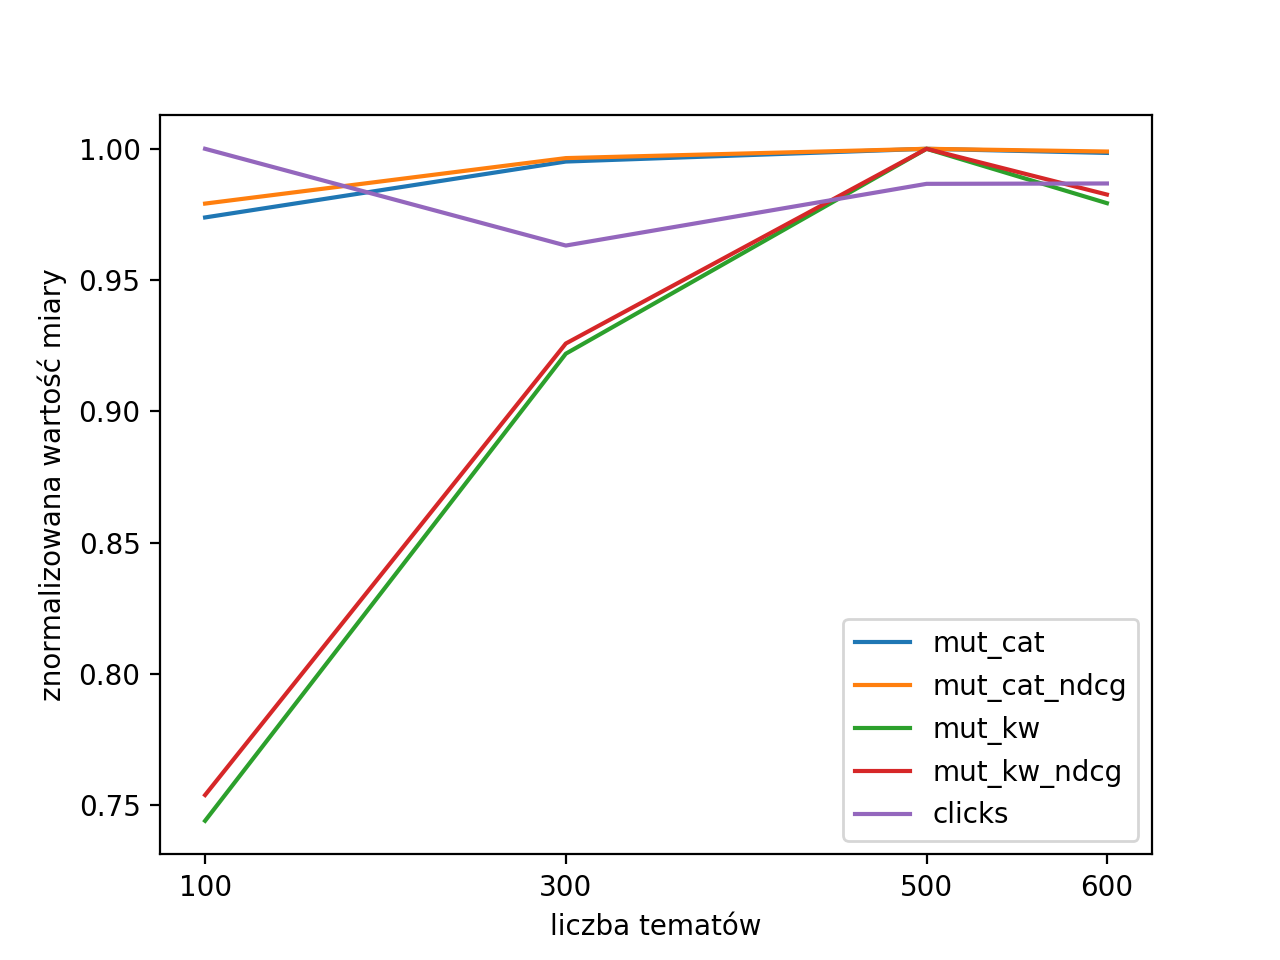
\includegraphics[width=1\textwidth]{img/results/lsi_.png}
		\end{figure}
	\end{frame}
	\begin{frame}{LDA w zależności od liczby tematów}
		\begin{figure}[H]
			\centering
			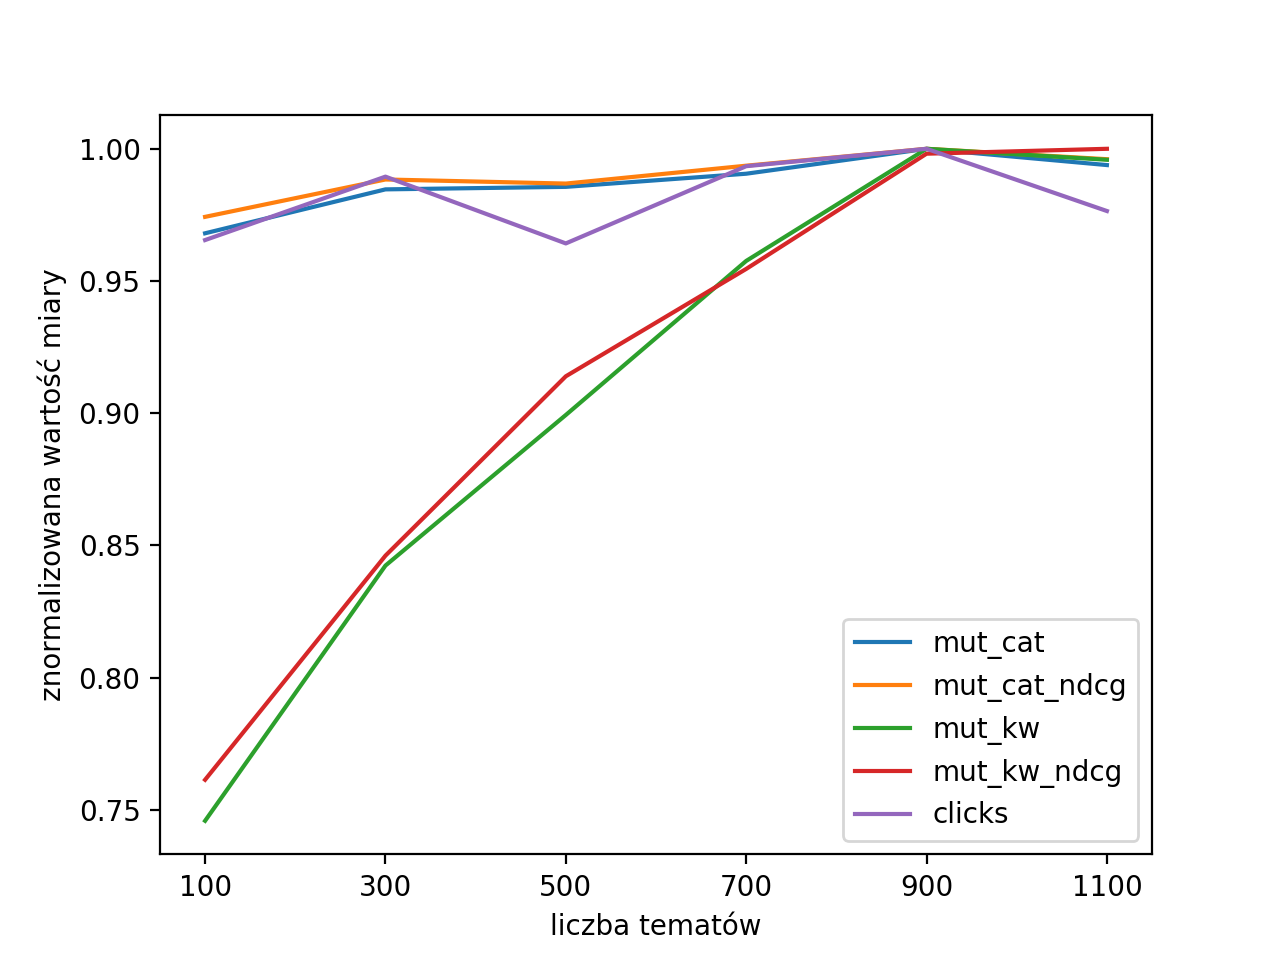
\includegraphics[width=1\textwidth]{img/results/lda_.png}
		\end{figure}
	\end{frame}
	\begin{frame}{Word2vec w zależności od korpusu}
		\begin{figure}[H]
			\centering
			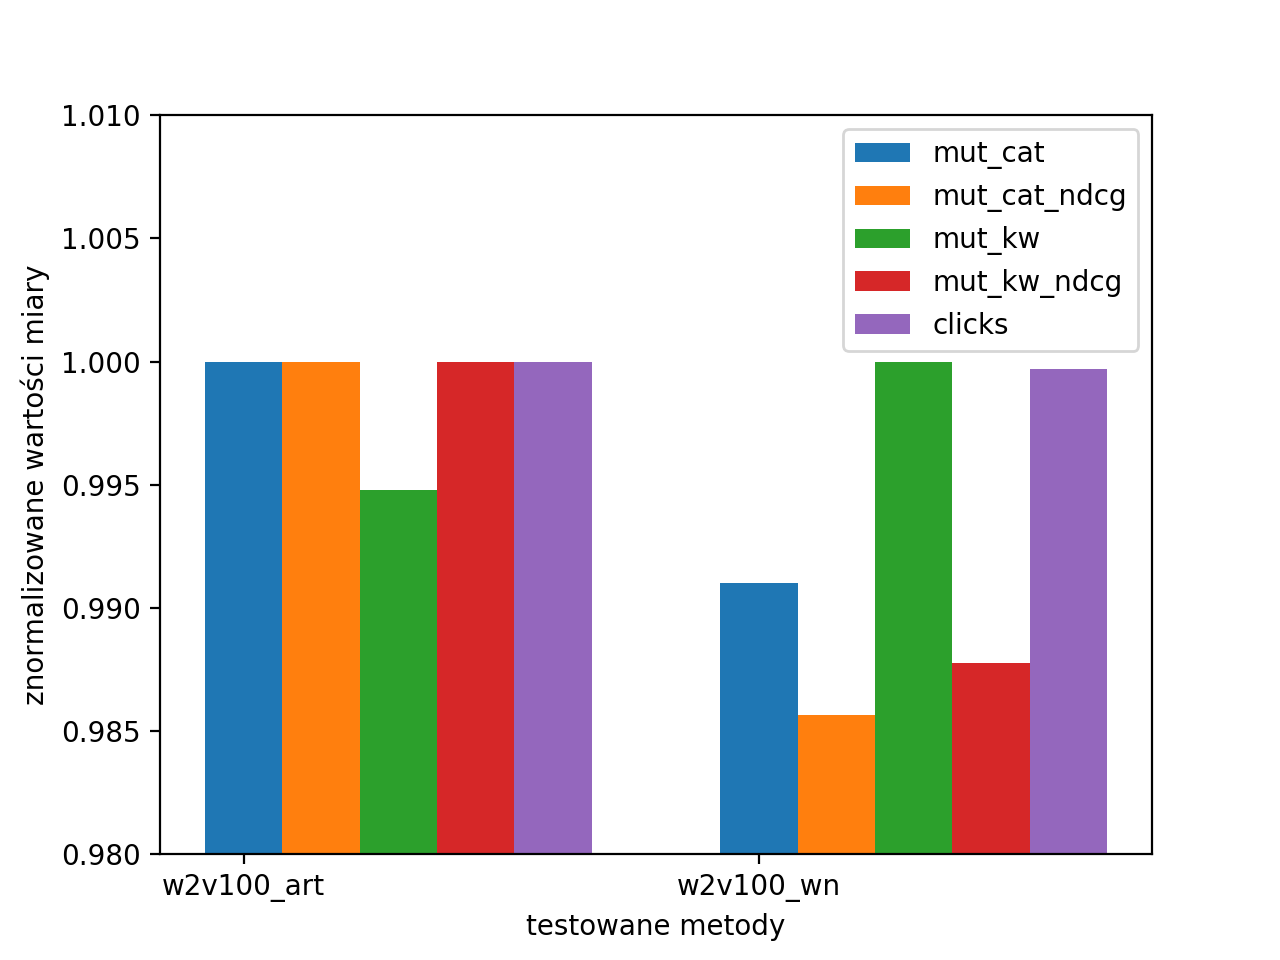
\includegraphics[width=1\textwidth]{img/results/w2v100_art_w2v100_wn_.png}
		\end{figure}
	\end{frame}
	\begin{frame}{Word2vec w zależności od długości wektorów}
		\begin{figure}[H]
			\centering
			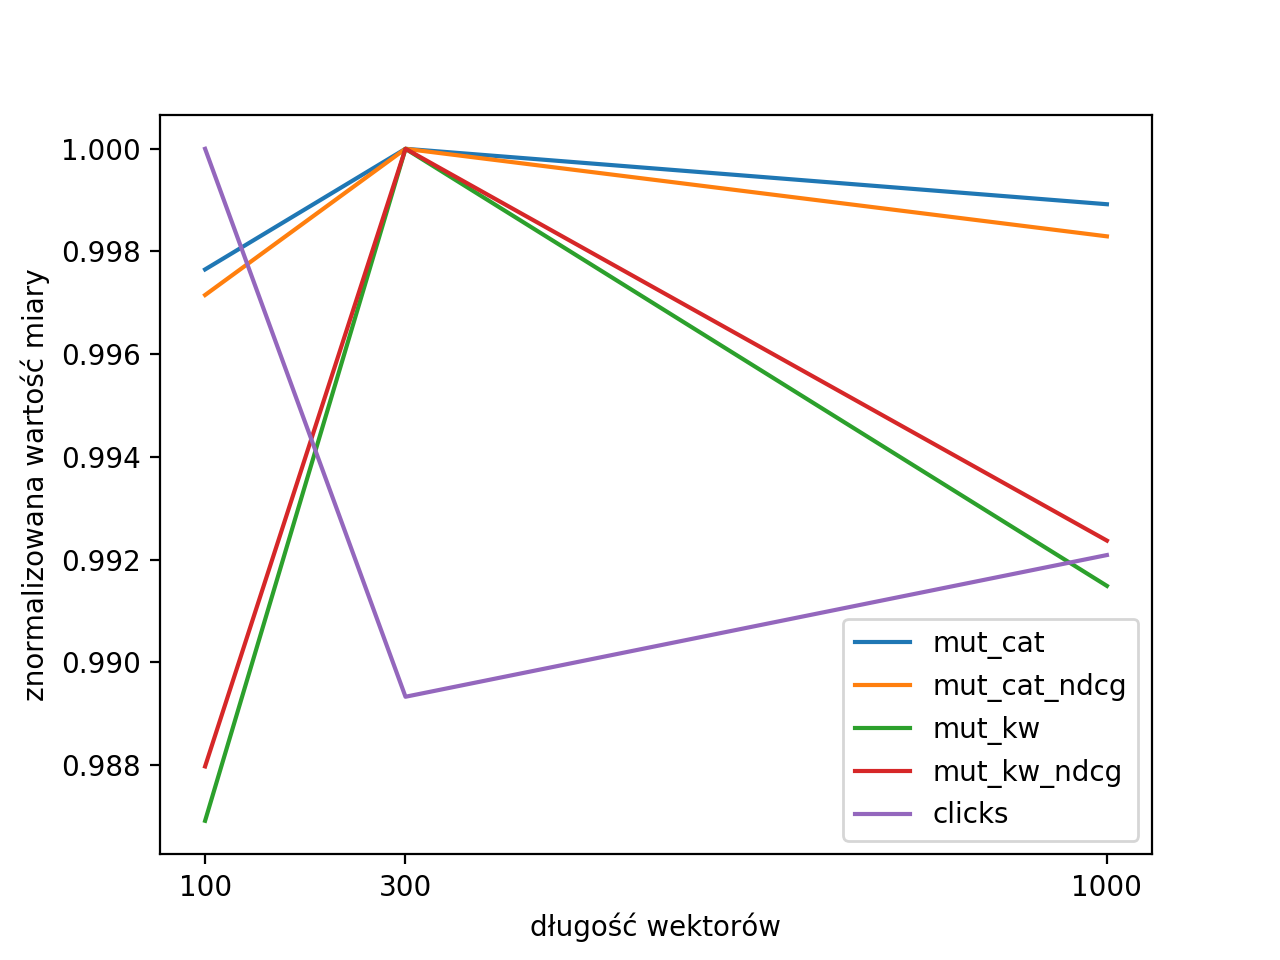
\includegraphics[width=1\textwidth]{img/results/w2v_ctr.png}
		\end{figure}
	\end{frame}
	\begin{frame}{GloVe w zależności od długości wektorów}
		\begin{figure}[H]
			\centering
			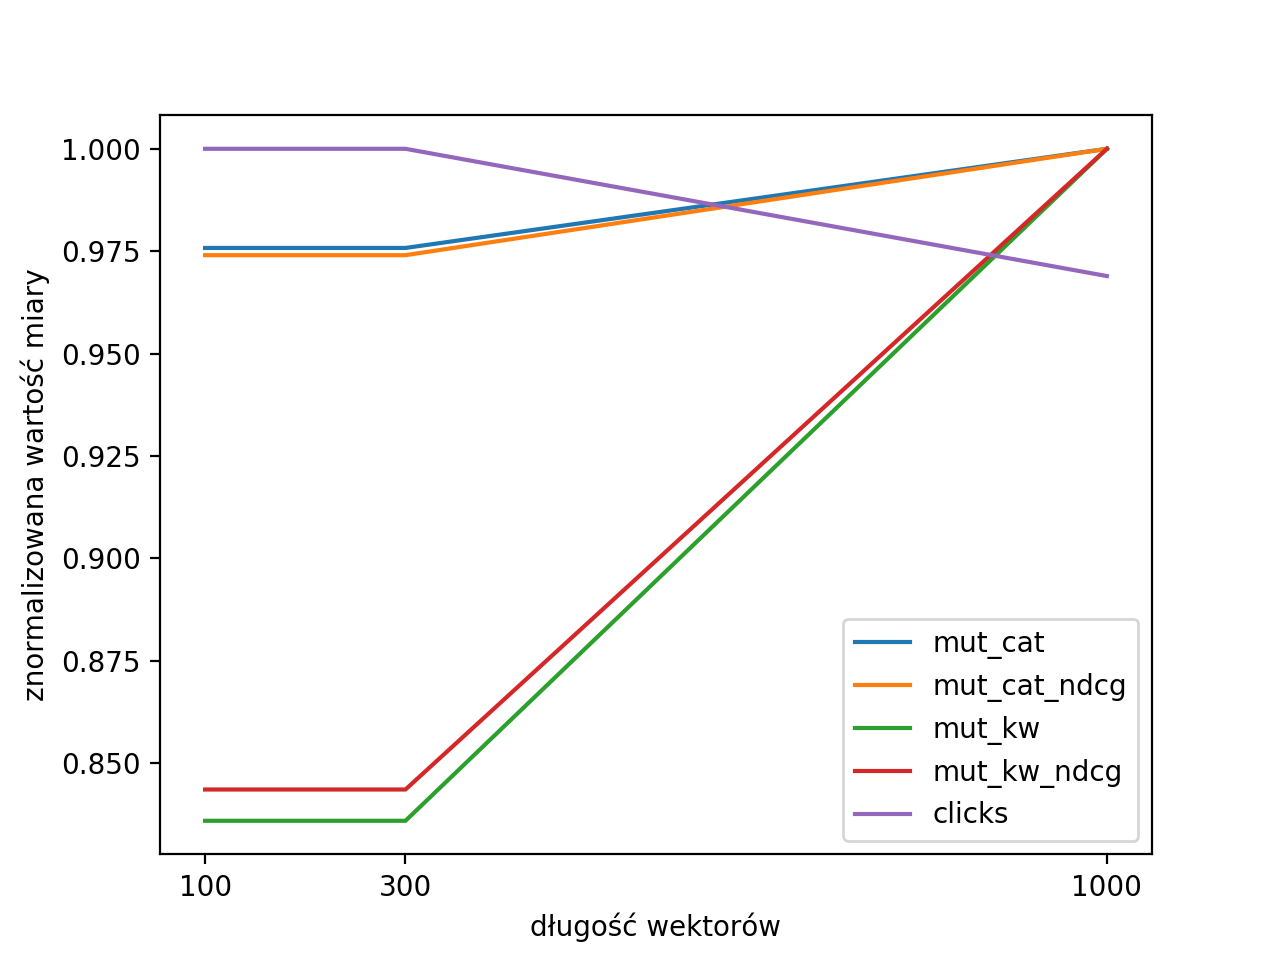
\includegraphics[width=1\textwidth]{img/results/gv_ctr.png}
		\end{figure}
	\end{frame}
	\begin{frame}{FastText w zależności od długości wektorów}
		\begin{figure}[H]
			\centering
			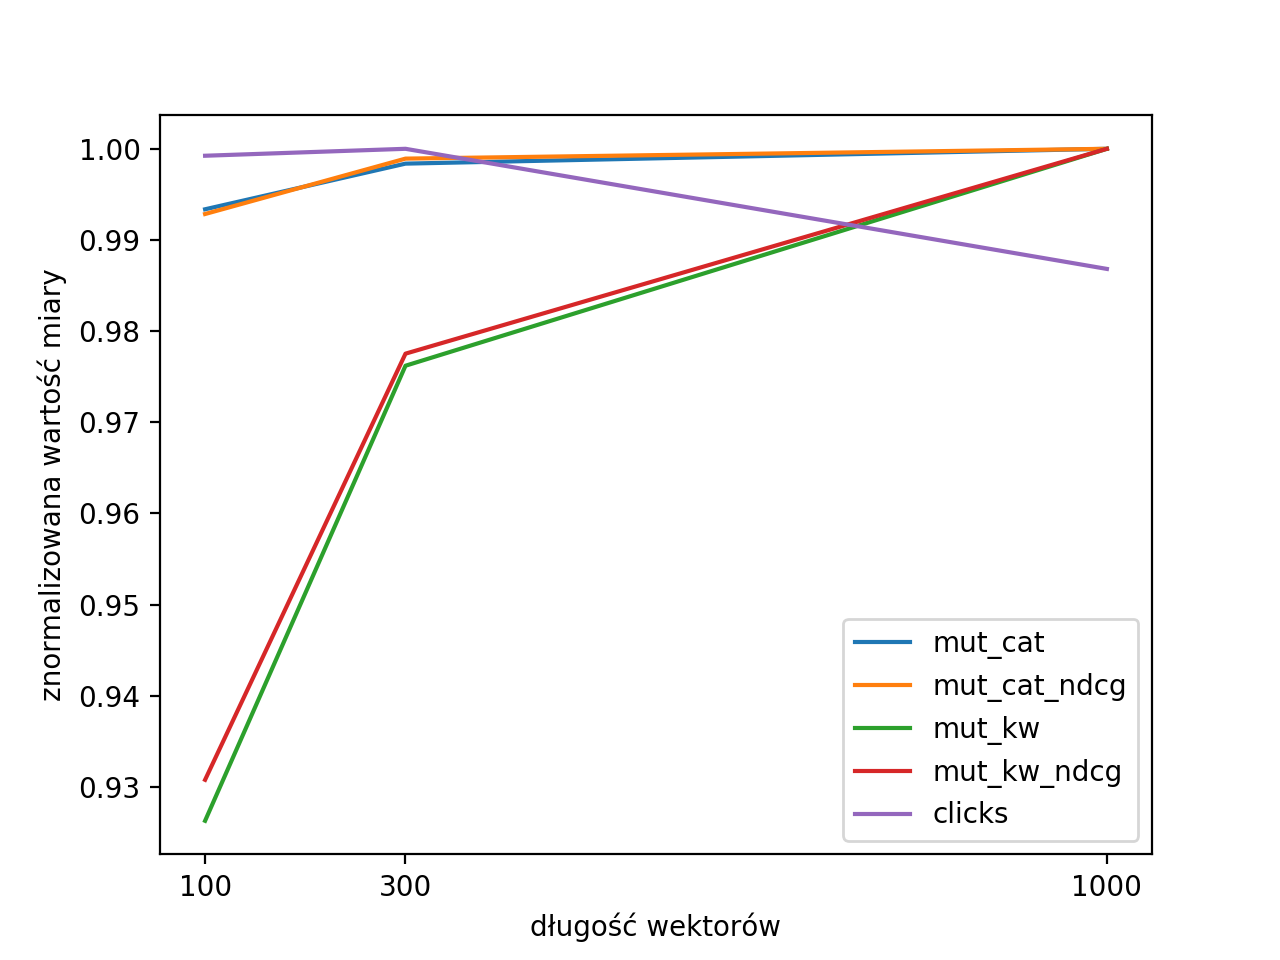
\includegraphics[width=1\textwidth]{img/results/ft_ctr.png}
		\end{figure}
	\end{frame}
	\begin{frame}{Wyniki ewaluacji eksperckiej dla~wybranych metod}
		\begin{figure}[H]
			\centering
			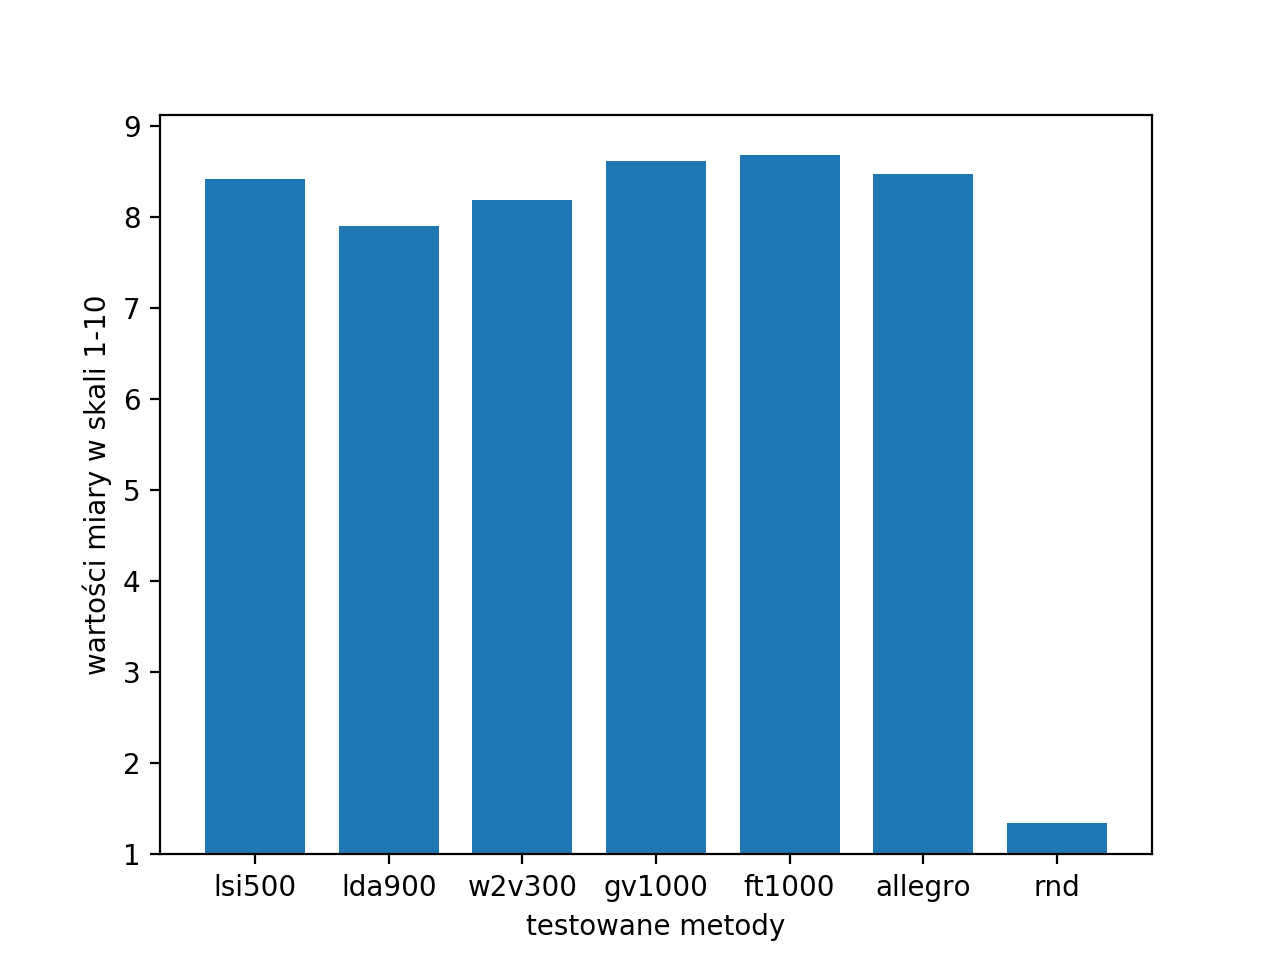
\includegraphics[width=0.8\textwidth]{img/results/lsi500_lda900_w2v300_gv1000_ft1000_allegro_rnd_users.png}
		\end{figure}
	\end{frame}
	\begin{frame}{Porównanie odchyleń standardowych ocen eksperckich dla~wybranych metod}
		\begin{figure}[H]
			\centering
			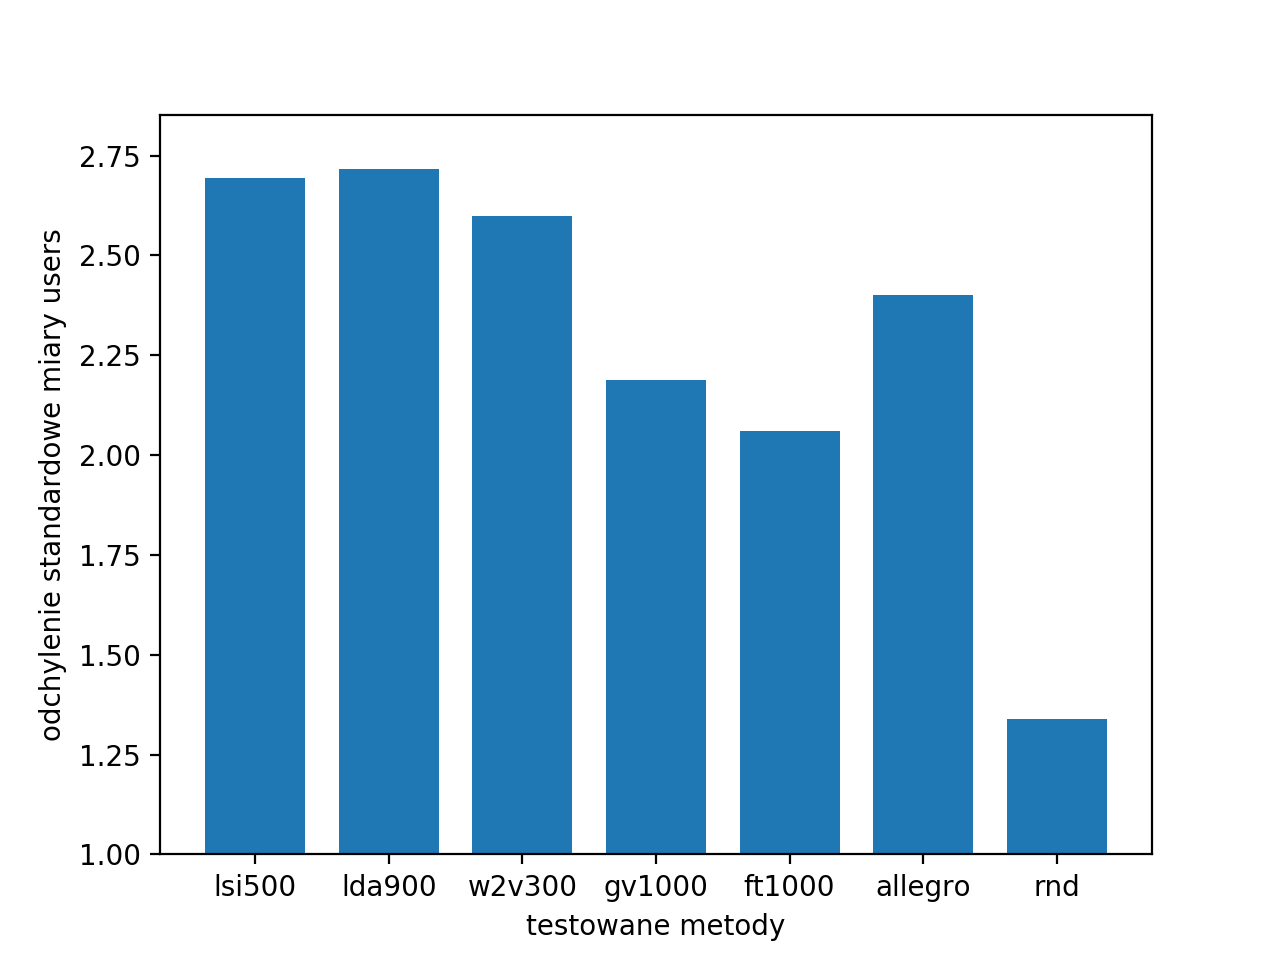
\includegraphics[width=0.8\textwidth]{img/results/lsi500_lda900_w2v300_gv1000_ft1000_allegro_rnd_users_std.png}
		\end{figure}
	\end{frame}
	\section{Podsumowanie}
	\begin{frame}{Podsumowanie testów}
		\begin{itemize}
			\item Brak istotnych statystycznie różnic między wynikami wszystkich metod \pause
			\item Im dłuższe wektory \emph{word embeddings} tym lepsze rezultaty \pause
			\item Większa liczba tematów nie implikuje lepszych rezultatów \pause
			\item ...
		\end{itemize}
	\end{frame}
	\begin{frame}{Kiernki dalszych badań}
		
	\end{frame}
	\begin{frame}{Wnioski}
		testowane metody nie odbiegają jakością od dotychczasowej.
		python
		elasticsearch
		nlp
		trudno jest zmierzyc efekty
	\end{frame}
	\section{Wybrane źródła}
	\begin{frame}{Wybrane źródła}
		\begin{thebibliography}{30}
			\bibitem{lda}
				D. M. Blei, A. Y. Ng, M. I. Jordan,
				\emph{Latent Dirichlet Allocation},
				Journal of Machine Learning Research, tom 3 num. 4–5,
				2003
			\bibitem{lsa}
				S. Deerwester, S. T. Dumais, G. W. Furnas, T. K. Landauer, R. Harshman,
				\emph{Indexing by latent semantic analysis},
				Journal of the American Society for Information Science, tom 41, num. 6,
				1990
			\bibitem{fasttext}
				A. Joulin, E. Grave, P. Bojanowski T. Mikolov,
				\emph{Bag of Tricks for Efficient Text Classification},
				Facebook AI Research,
				2016
			\bibitem{word2vec}
				T. Mikolov, K. Chen, G. Corrado, J. Dean,
				\emph{Efficient Estimation of Word Representations in Vector Space},
				International Conference on Machine Learning (ICML),
				2013
			\bibitem{glove}
				J. Pennington, R. Socher, C. D. Manning,
				\emph{GloVe: Global Vectors for Word Representation},
				Computer Science Department, Stanford University, Stanford, CA 94305,
				2014
		\end{thebibliography}
	\end{frame}
\end{document}
